\documentclass[a4paper]{article}
\usepackage[ngerman]{babel}
\usepackage[T1]{fontenc}
\usepackage[utf8]{inputenc}
\usepackage{textcomp}
\usepackage{geometry}
\geometry{ left=2cm, right=2cm, top=2cm, bottom=4cm, bindingoffset=5mm}
\usepackage{graphicx}
\usepackage{xcolor}
\usepackage{hyperref}
\date{}
\author{}
\usepackage{fancyhdr}
\pagestyle{fancy}
\fancyhf{}
\fancyhead[R]{3141241 - Jamie Ullerich \\ 2892258 - Gerhard Breul \\ 2973140 - Felix Bühler}
\fancyhead[L]{Information Visualisation and Visual Analytics \\ WS 2019/20 }
\renewcommand{\headrulewidth}{0.5pt}
\usepackage{tikz}
\usetikzlibrary{calc}
\usepackage{amsmath}


\title{\textbf{Assignment 5}}

\begin{document}
\maketitle 
\thispagestyle{fancy}

\section*{Task 1 - Trees}
\subsection*{a)}
\begin{enumerate}
	\item Parent nodes/folders are clearly visible as all children are alligned in the same row.
	\item Every node in an indented tree can be easily labeled.
\end{enumerate}
\subsection*{b)}
One way to incorporate a folder's size into its representation in the indented tree is to color code each node according to its relative disk usage. The darker the color, the bigger the corresponding folder or file.\\
Another Possibility is to represent memory usage as a bar under or next to the corresponding file, effectively adding a horizontal bar graph to the indented tree. While this would (depending on the graph's scale) showcase size more accurately, the size of very small files might become difficult to assess.
\subsection*{c)}



\section*{Task 2 - Tree-Maps with Slice \& Dice}
\begin{figure}[!ht]
	\centering
	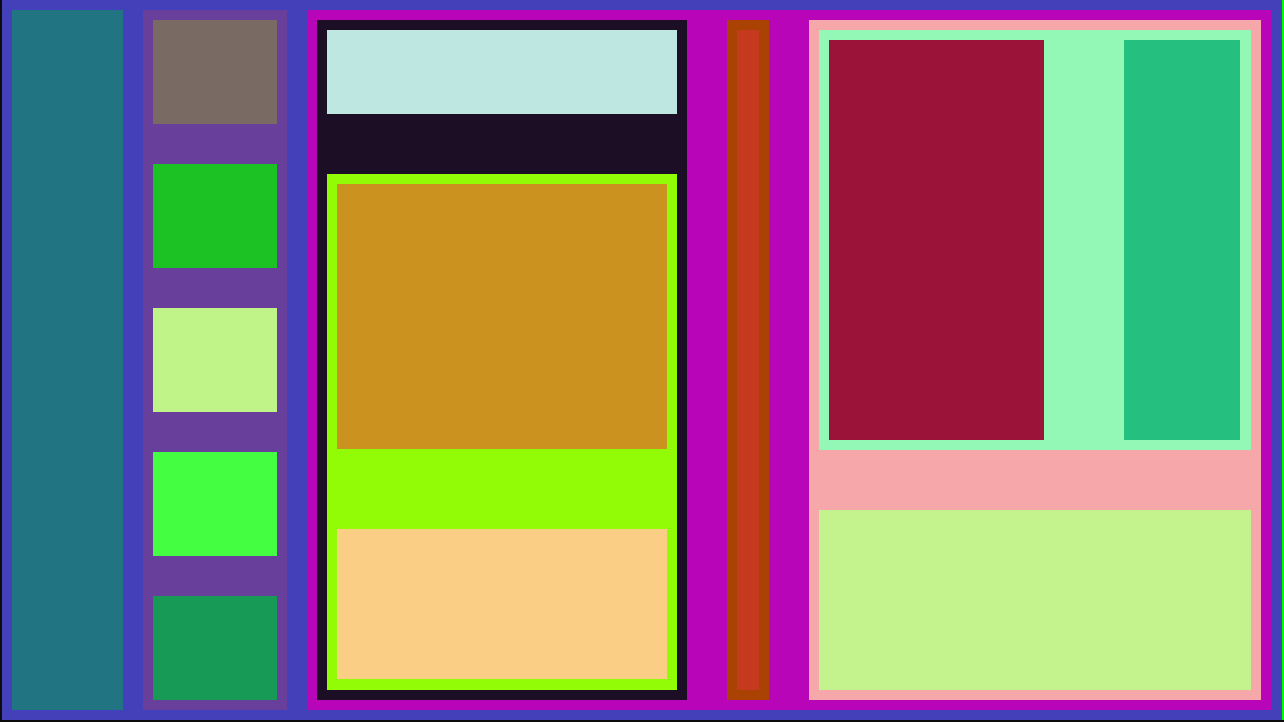
\includegraphics[width=0.9\linewidth]{5_2}
	\caption{Solution}
\end{figure}


\end{document}
